\documentclass[10pt, compress]{beamer}

\usetheme{m}

\usepackage{booktabs}
\usepackage[scale=2]{ccicons}
\usepackage{minted}
\usepackage{tikz}
\usetikzlibrary{calc, arrows}
\usepackage{xstring}
\usepackage{amsmath}
\usepgfplotslibrary{dateplot}
\usemintedstyle{trac}


\usetikzlibrary{shapes,arrows}
\tikzstyle{cloud} = [draw, ellipse, node distance=4cm,    minimum height=2em]
\tikzstyle{cloudgreen} = [draw, ellipse, fill=green!20, node distance=4cm,    minimum height=2em]
\tikzstyle{blockred} = [rectangle, draw, fill=red!20, 
text width=5em, text centered, rounded corners, minimum height=4em, minimum width= 6em]
\tikzstyle{block} = [rectangle, draw, fill=white!20, 
text width=5em, text centered, rounded corners, minimum height=4em,minimum width= 6em]
\tikzstyle{blockgreen} = [rectangle, draw, fill=green!20, 
text width=5em, text centered, rounded corners, minimum height=4em, minimum width= 6em]
\tikzstyle{line} = [draw, -latex']


\renewcommand{\(}{\begin{columns}}
\renewcommand{\)}{\end{columns}}
\newcommand{\<}[1]{\begin{column}{#1}}
	\renewcommand{\>}{\end{column}}
%%%%%%%%%%%%%%%%%%%%%%%%%%%%%%%%%%%%%%%%%%%%%%%%%%
\newcommand*{\NodeSize}{0.5cm}%
\newcommand*{\YShiftBetweenRows}{-1cm}% Subsequent rows are shited down so they don't overlap
\tikzset{DNA Style/.style={minimum size=0.5cm, draw=gray, line width=1pt}}{}

\newlength{\YShift}% 
\newcounter{ColumnCounter}% Prefix for node labels

% Initialize - These are probably not needed, but prefer to set them
\setlength{\YShift}{0cm}% 
\setcounter{ColumnCounter}{0}
\newcommand*{\DNASequence}[2][Mark]{%
	% http://tex.stackexchange.com/questions/12091/tikz-foreach-loop-with-macro-defined-list
	\def\Sequence{#2}
	\foreach [count=\xi] \Label/\Color in \Sequence {%
		\pgfmathsetmacro{\XShift}{\NodeSize*\xi}%
		\IfStrEq{\Color}{}{\def\Color{white}}{}
		\edef\NodeName{#1-\arabic{ColumnCounter}}
		\node [DNA Style, fill=\Color, xshift=\XShift] (\NodeName) {\Label};
		\stepcounter{ColumnCounter}
	} 
}%
\newcommand*{\ThreeDNASequences}[4][Mark]{% #1 = tikzmark prefix
	\setcounter{ColumnCounter}{0}% reset column counter
	\begin{scope}[yshift=\YShift]
		\DNASequence[#1]{#2} 
		\pgfmathsetmacro{\Shift}{6cm}% Should compute this based on num of items in #1
		\begin{scope}[xshift=\Shift]
			\DNASequence[#1]{#3} 
		\end{scope}
		\pgfmathsetmacro{\Shift}{8cm}% Should compute this based on num of items in #2  
		\begin{scope}[xshift=\Shift]
			\DNASequence[#1]{#4} 
		\end{scope}
	\end{scope}
	\pgfmathsetlength{\YShift}{\YShift\YShiftBetweenRows}%
}

\title{Human Genetic Variation Viewer}
%\subtitle{}

\vspace*{20pt}
\author[skc]{Saket Choudhary \inst{1}, Leyla Garcia\inst{2} and Andrew Nightingale\inst{2}}
\institute{\inst{1} University of Southern California and \inst{2} EMBI-EBI}

\date{\vspace*{50pt}
    \begin{center}
        \today \\
        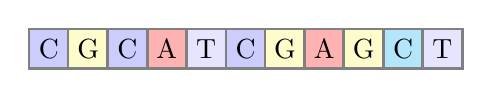
\begin{tikzpicture}
        \DNASequence[Top]{C/blue!20,G/yellow!20,C/blue!20, A/red!30,T/blue!10,C/blue!20, G/yellow!20,A/red!30, G/yellow!20,C/cyan!30,T/blue!10}; 
        \end{tikzpicture}
        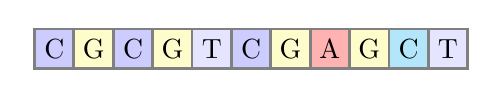
\begin{tikzpicture}
        \hspace*{2pt}\DNASequence[Bottom]{C/blue!20,G/yellow!20,C/blue!20,G/yellow!20,T/blue!10,C/blue!20, G/yellow!20,A/red!30, G/yellow!20,C/cyan!30,T/blue!10}; 
        \end{tikzpicture}
    \end{center}
}

\begin{document}

\maketitle


\begin{frame}[fragile]
\frametitle{Outline}
\begin{itemize}
\item Motivation
\item Solution
%\item BioJS and re-usability
\item Demo and Use-Cases
\item Implementation
\item Improvements
\end{itemize}
\end{frame}

\section{Motivation}


\begin{frame}[fragile]
  \frametitle{Visualizations are powerful!}
    \begin{quote}
        The power of the unaided mind is highly overrated. The real
        powers come from devising external aids that enhance
        cognitive abilities. 
        -- Donald Norman
    \end{quote}
\end{frame}





\begin{frame}[fragile]
  \frametitle{Motivation}
  \begin{itemize}[<+- | alert@+>]
	  \item NGS has given rise to catalog of genetic variants: dbSNP, COSMIC...
	  \item Loads of data, but limited relevant information: Benign, Damaging, Intermediate
	  \item Lots of mutations $\implies$ Loads of \emph{differing} predictions
	  \item Non consensus scoring mechanisms: SIFT and Polyphen predictions for example can be entirely opposite
	  \item Exploratory visualization is the first step towards discovering patterns
	  \item Variation viewers are \emph{absent}, if not, provide limited flexibility
	  %Too many SNPs, too many 'drivers'
  \end{itemize}
  

\end{frame}


\begin{frame}[fragile]
\frametitle{Solution}

  \begin{itemize}[<+- | alert@+>]
    %\item \alert<4>{This is\only<4>{ really} important}
    %\item Pool data, visualize, discover
    \item A graphical hub to present annotated variants from different sources
   	\item Present information at different levels in a coherent manner
   	\item Scalable,  and Interactive exploration on the browser
   	
  \end{itemize}
\end{frame}


\plain{Demo \\ \url{http://saketkc.github.io}}


\section{Details}

\begin{frame}
\frametitle{Implementation}
\begin{itemize}[<+- | alert@+>]
\item Entirely written in javascript using the \textit{d3js} library
\item Deployed as a BioJS component
\item Events system that triggers events on user actions, allows cross-component communication

 \end{itemize}
\end{frame}

\begin{frame}
\frametitle{Why BioJS}
\begin{itemize}[<+- | alert@+>]
\item BioJS is a javascript library for developing visualization of the biological data
\item 
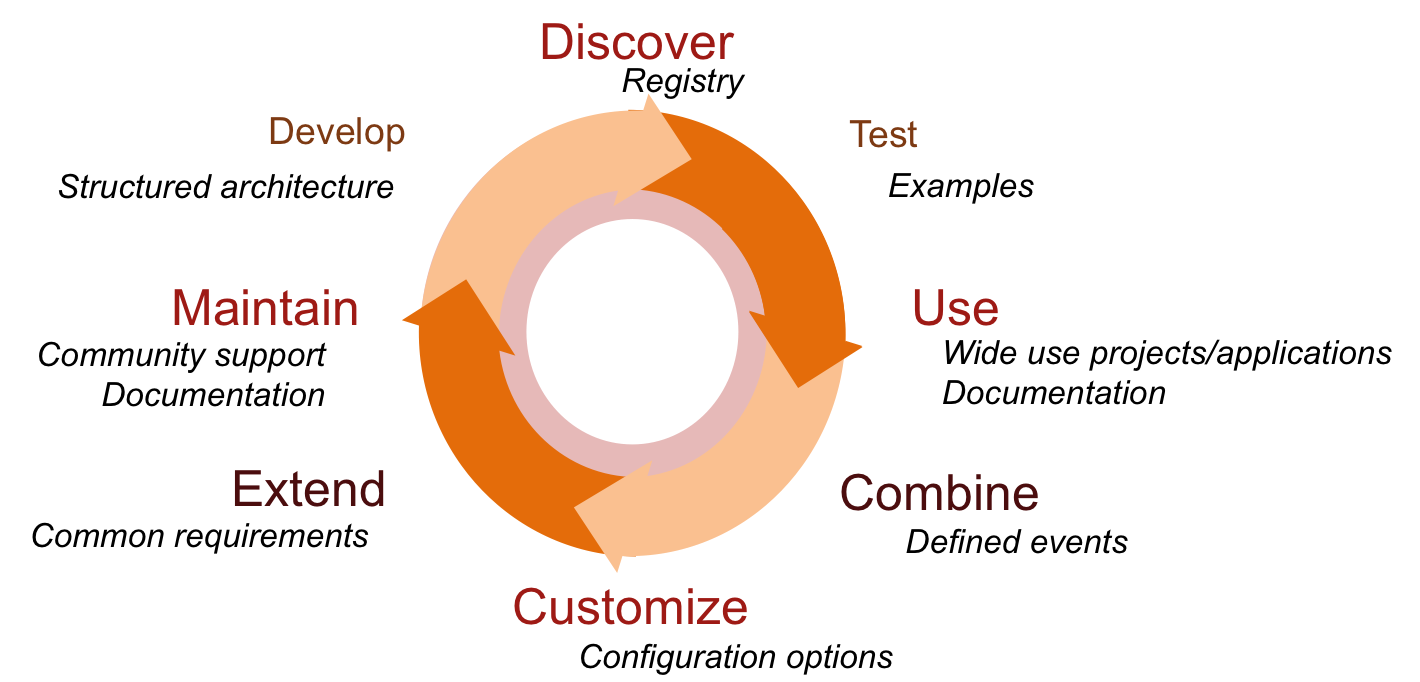
\includegraphics[width=\linewidth]{images/cycle}

\end{itemize}
\end{frame}

\begin{frame}
\frametitle{Why BioJS}
%\begin{itemize}[<+- | alert@+>]
%\item 
Reusable components that can talk to each other
%\item 
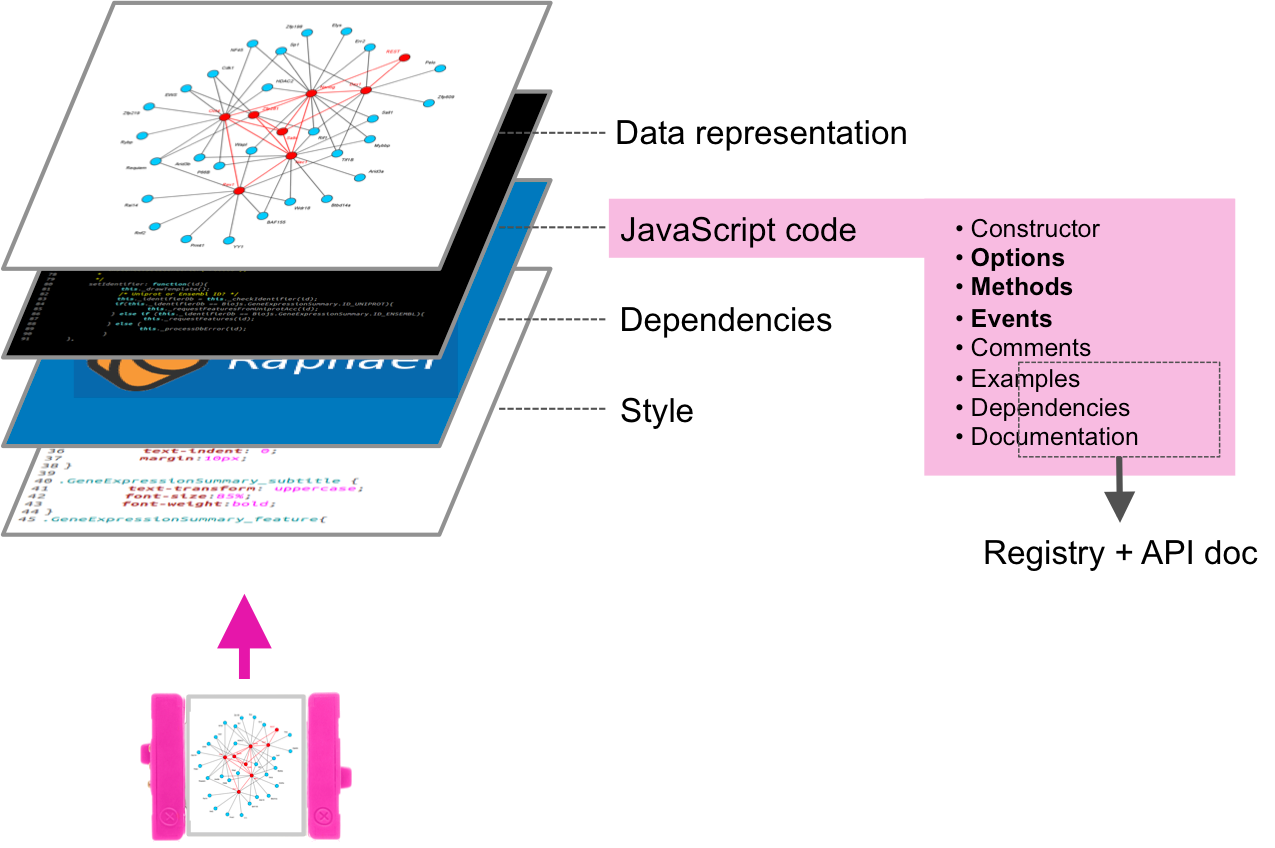
\includegraphics[scale=0.15]{images/biojs_component_layers}\\
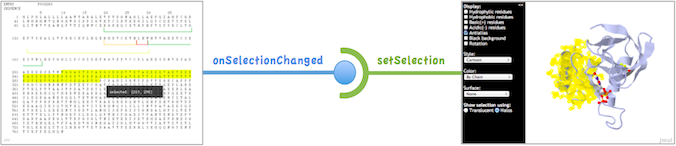
\includegraphics[width=\linewidth]{images/biojs_events}
%\end{itemize}
\end{frame}




\begin{frame}[fragile]
\frametitle{Data Input}
\begin{minted}{json}
{
"id":"P00533_variant226",
"sourceIds":["COSM1090877","COSM1090879"],
"position":541,
"wild_type":"L",
"mutation":"I",
"frequency":0.0,
"polyphenPrediction":"benign",
"polyphenScore":0.0,
"siftPrediction":"tolerated",
"siftScore":0.86,
"somaticStatus":1,
"consequenceTypes":"missense variant",
"cytogeneticBand":"7p11.2",
"genomicLocation":"7:g.55229314C>A"
}
\end{minted}
\end{frame}

\begin{frame}[fragile]
\frametitle{Data Input}
\begin{itemize}
\item Pre-generated JSON files
\item Current version uses files generated by an unpublished webservice at EBI
\item Protein variants, though not specific to it
\end{itemize}
\end{frame}


\begin{frame}{Features}
\begin{itemize}
\item Supports JSON formatted files, alpha VCF support
\item User defined scoring criteria
\item Different levels of information
\begin{itemize}
\item Overview: Condensed information
\item Zoomed View: All annotations 
\end{itemize}
\item Loading proteins through URL parameters
\item SIFT, Polyphen, ....

\end{itemize}
\end{frame}

\begin{frame}
\frametitle{Use Cases}
\begin{itemize}[<+- | alert@+>]
\item Identifying most or least mutated sites across proteins
\item Discover differences between different scoring criteria
\item Benchmarking predictions
\end{itemize}

\end{frame}

\begin{frame}
\frametitle{Improvements}
\begin{itemize}[<+- | alert@+>]
\item VCF support(almost there)
\item Integration with Galaxy, web based bioinformatics workflows
\item Performance improvements
\item Interaction with 3D Protein viewer to highlight domains
\end{itemize}
\end{frame}

\section{Conclusion}

\begin{frame}{Summary}
\begin{itemize}
\item A tool for visualizing genetic variants
\item Supports visualization of different levels of information
\item Cross component talks
\item User defined and user controlled

\end{itemize}

\end{frame}

\begin{frame}
\frametitle{Acknowledgements}
Google, for running the Google Summer of Code 2014.
\end{frame}

\plain{Questions?}

\end{document}
